%%
\section{Data Samples}
\label{sec:data}

This analysis has been performed on proton-proton collision data with a center-of-mass energy of 8 TeV collected with the CMS detector. The dataset used is /SinglePhotonParked/Run2012D-22Jan2013-v1/AOD with an integrated luminosity of $7.3 \fbinv$.

The recommended noise event filters are applied to ensure good quality of data. More details on these filters can be found in \cite{CMS_AN_2012-268}. The recommended noise event filters are as follows:

\begin{itemize}
\item CSC tight beam halo: rejects events with a secondary particle shower produced due to collisions of the beam with residual gas inside the LHC vacuum chamber.
\item HBHE noise filter: removes events with noise in the hybrid photo-diodes (HPTDs), used to convert the scintillator light into an electrical output and the readout boxes (RBXs) which contain them.
\item ECAL dead cell trigger primitive (TP) filter: rejects events where the TP \et at the masked crystal cells exceed 63.75 GeV
\item HCAL laser filter: rejects events when misfiring of the HCAL laser at a wrong time (when proton bunches collide) was observed. 
\item Tracking failure filter: rejects events where standard or large calorimetry deposits contrast with a lack of reconstructed tracks.
\item Bad EE Supercrystal filter: removes events from two EE 5x5 crystals that give anomalously high energy.
\item Tracking POG filters: reject sevents where no tracks are reconstructed due to aborting of the reconstruction algorithm because of CPU time limits.
\end{itemize}

%%
\section{Monte Carlo Samples}
\label{sec:mc}

Monte Carlo (MC) event generators are used to simulate the signal and background processes. The different processes were simulated using the \MADGRAPH~\cite{madgraph}, and \PYTHIA~\cite{pythia} generators with the parton fragmentation and hadronization being done by \PYTHIA. The detailed list of the simulated samples used for signal and background processes and their respective cross sections are shown in Table ~\ref{table:mcsample}. 

\begin{table}[!h]
  \centering
  \caption{MC samples used in the analysis (AOD).}
  \label{table:mcsample}         
  \scalebox{0.65}{
    \begin{tabular}{|l|l|c|c|}
      \hline
      Process & Sample Name  & X\-Sec (pb) & Lumi ($\fbinv$)\\
      \hline
      \hline
      $\gamma\gamma$ + j & /DiPhotonJets\_8TeV-madgraph-tarball-v2/Summer12\_DR53X-PU\_S10\_START53\_V7A-v1 & 1.0 & 10$^{3}$ \\
      $\gamma\gamma$ & /DiPhotonBox\_Pt-*To*\_8TeV-pythia6/Summer12\_DR53X-PU\_S10\_START53\_V7A-v1 & 0.00032-15.5 & 32-10$^{6}$ \\
      W($\to$ l $\nu$)$\gamma$ & /WGToLNuG\_TuneZ2star\_8TeV-madgraph-tauola/Summer12\_DR53X-PU\_S10\_START53\_V7A-v1 & 461.6 & 10.8 \\
      Z($\to$ $\nu$ $\nu$)$\gamma$ & /ZG\_Inclusive\_8TeV-madgraph/Summer12\_DR53X-PU\_S10\_START53\_V7A-v1 & 123.9 & 25.5 \\
      Z($\to$ l l)$\gamma$ & /ZGToLLG\_8TeV-madgraph/Summer12\_DR53X-PU\_S10\_START53\_V7A-v1/AODSIM & 132.6 & 49.6\\ 
      W $\to$ $\tau$ $\nu$ & /WToTauNu\_TuneZ2star\_8TeV\_pythia6\_tauola\_cff/Summer12\_DR53X-PU\_S10\_START53\_V7A-v1 & 9170 & 0.545 \\
      W $\to$ e $\nu$ &/WToENu\_TuneZ2star\_8TeV\_pythia6/Summer12\_DR53X-PU\_S10\_START53\_V7A-v2 & 9170 & 0.532 \\
      W $\to$ $\mu$ $\nu$ &/WToMuNu\_TuneZ2star\_8TeV\_pythia6/Summer12\_DR53X-PU\_S10\_START53\_V7C-v1 & 9170 & 0.52 \\
      DY $\to$ ee &/DYToEE\_M\_20\_TuneZ2star\_8TeV\_pythia6\_v2/Summer12\_DR53X-PU\_S10\_START53\_V7A-v1 & 1510.0 & YY \\
      $\gamma$ + j & /G\_Pt-*to*\_TuneZ2star\_8TeV\_pythia6/Summer12\_DR53X-PU\_S10\_START53\_V7A-v1 & 107.5-20930 & 0.9-89\\
      $\gamma$ + j & /GJets\_HT\-*To*\_8TeV\-madgraph/Summer12\_DR53X\-PU\_S10\_START53\_V19\-v1 & 107.5-20930 & 0.9-89\\
      \hline
      \hline
      Exotic Higgs & /GluGluToHToGam2Gravitino\_MChi*\_8TeV-calchep-pythia6/Summer12\_DR53X-PU\_S10\_START53\_V19 & 0.017 - 1.0 & - \\
      %Dark Matter & /BLA & XX & YY \\
      \hline
    \end{tabular}
  }
\end{table}

The exotic Higgs signal samples have been computed using the CalcHEP matrix element generator \cite{calchep},\cite{calchep2} and the corresponding choice of parameters are $m_\chi = 80$ GeV, BR($h\to \chi_1^0\tilde{G}$) = $2\times 10^{2}$ and BR($Z\to \chi_1^0\tilde{G}$) = $5\times 10^{6}$, where the SM Higgs and $Z$ boson total widths are used. The kinematic distribution for the signal can be seen in Figure~\ref{fig:signal_kinematics}

\begin{figure}[htb]
\begin{center}
{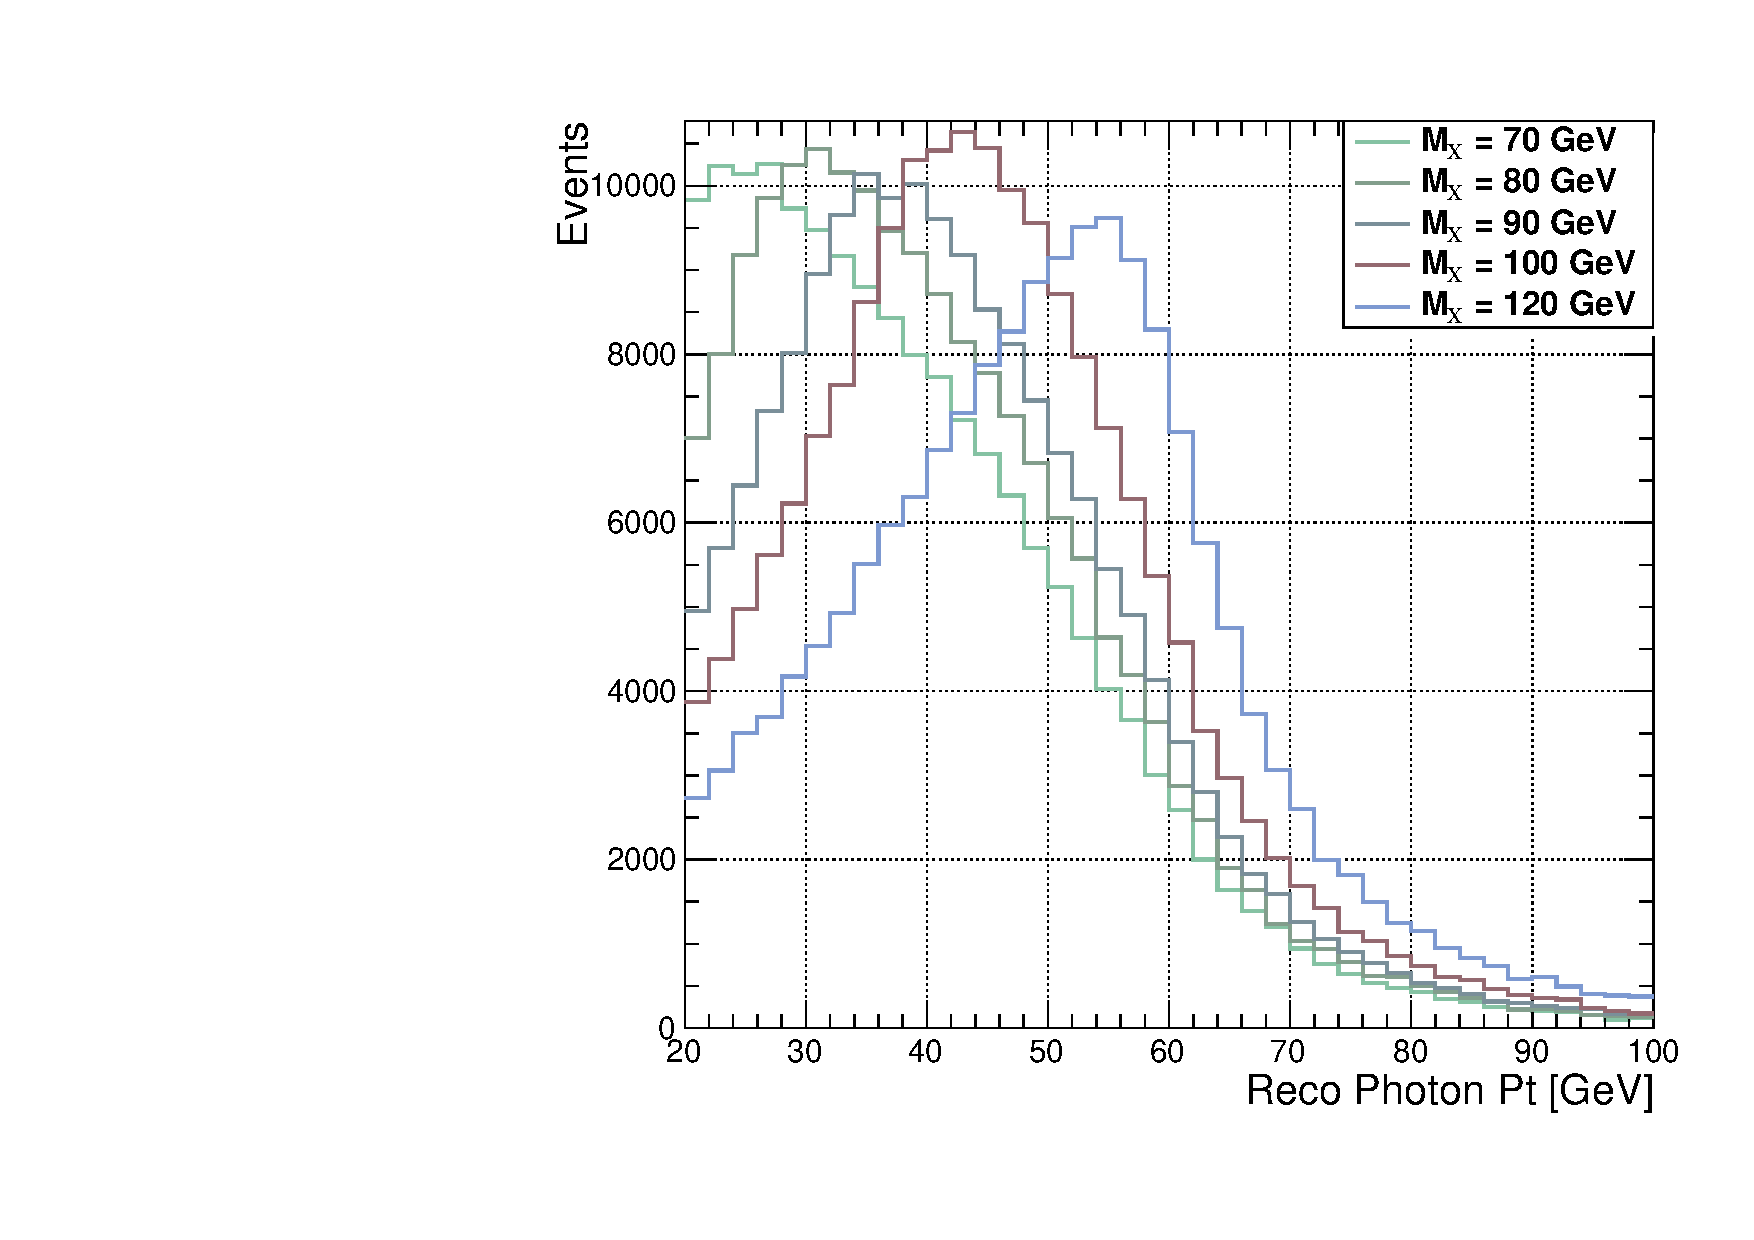
\includegraphics[width=0.45\textwidth]{analysis_figs/signal_photon.pdf}}\hfill
{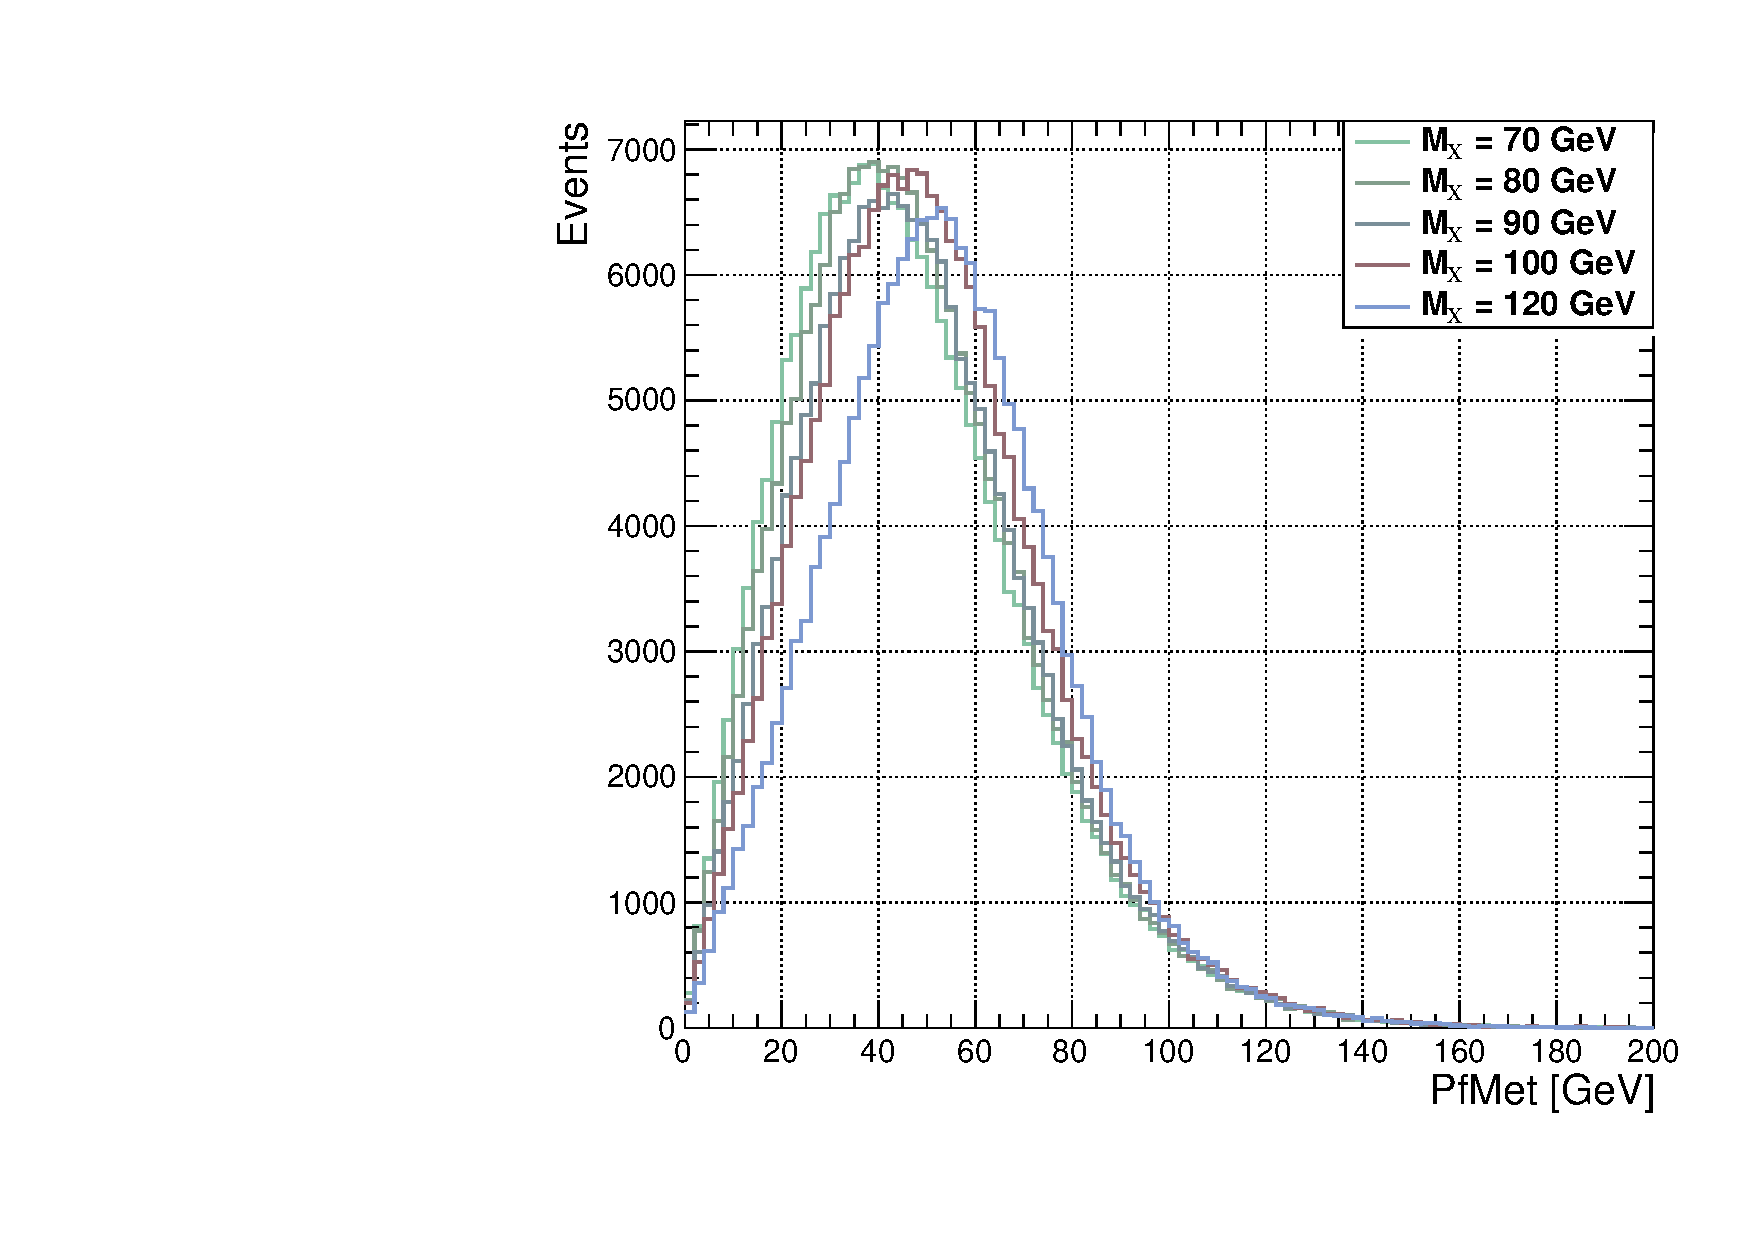
\includegraphics[width=0.45\textwidth]{analysis_figs/signal_met.pdf}}\hfill
\caption{Photon \ET and \met distribution for the Exotic Higgs Signal Model}
\label{fig:signal_kinematics}
\end{center}
\end{figure}

As mentioned the generation of the signal sample was done through CalcHep. At the LHE step, the Higgs \pt is 0 for all events because there is nothing recoiling off of the Higgs decay products. The Higgs pT distribution of the Higgs is given by \PYTHIA during the hadronization process and is then corrected using the differential cross section for Higgs boson as a function of generated Higgs boson \et shape coming from HRes generator. The difference in shape is shown in Figure~\ref{fig:shape_gen}. 

\begin{figure}[htb]
\begin{center}
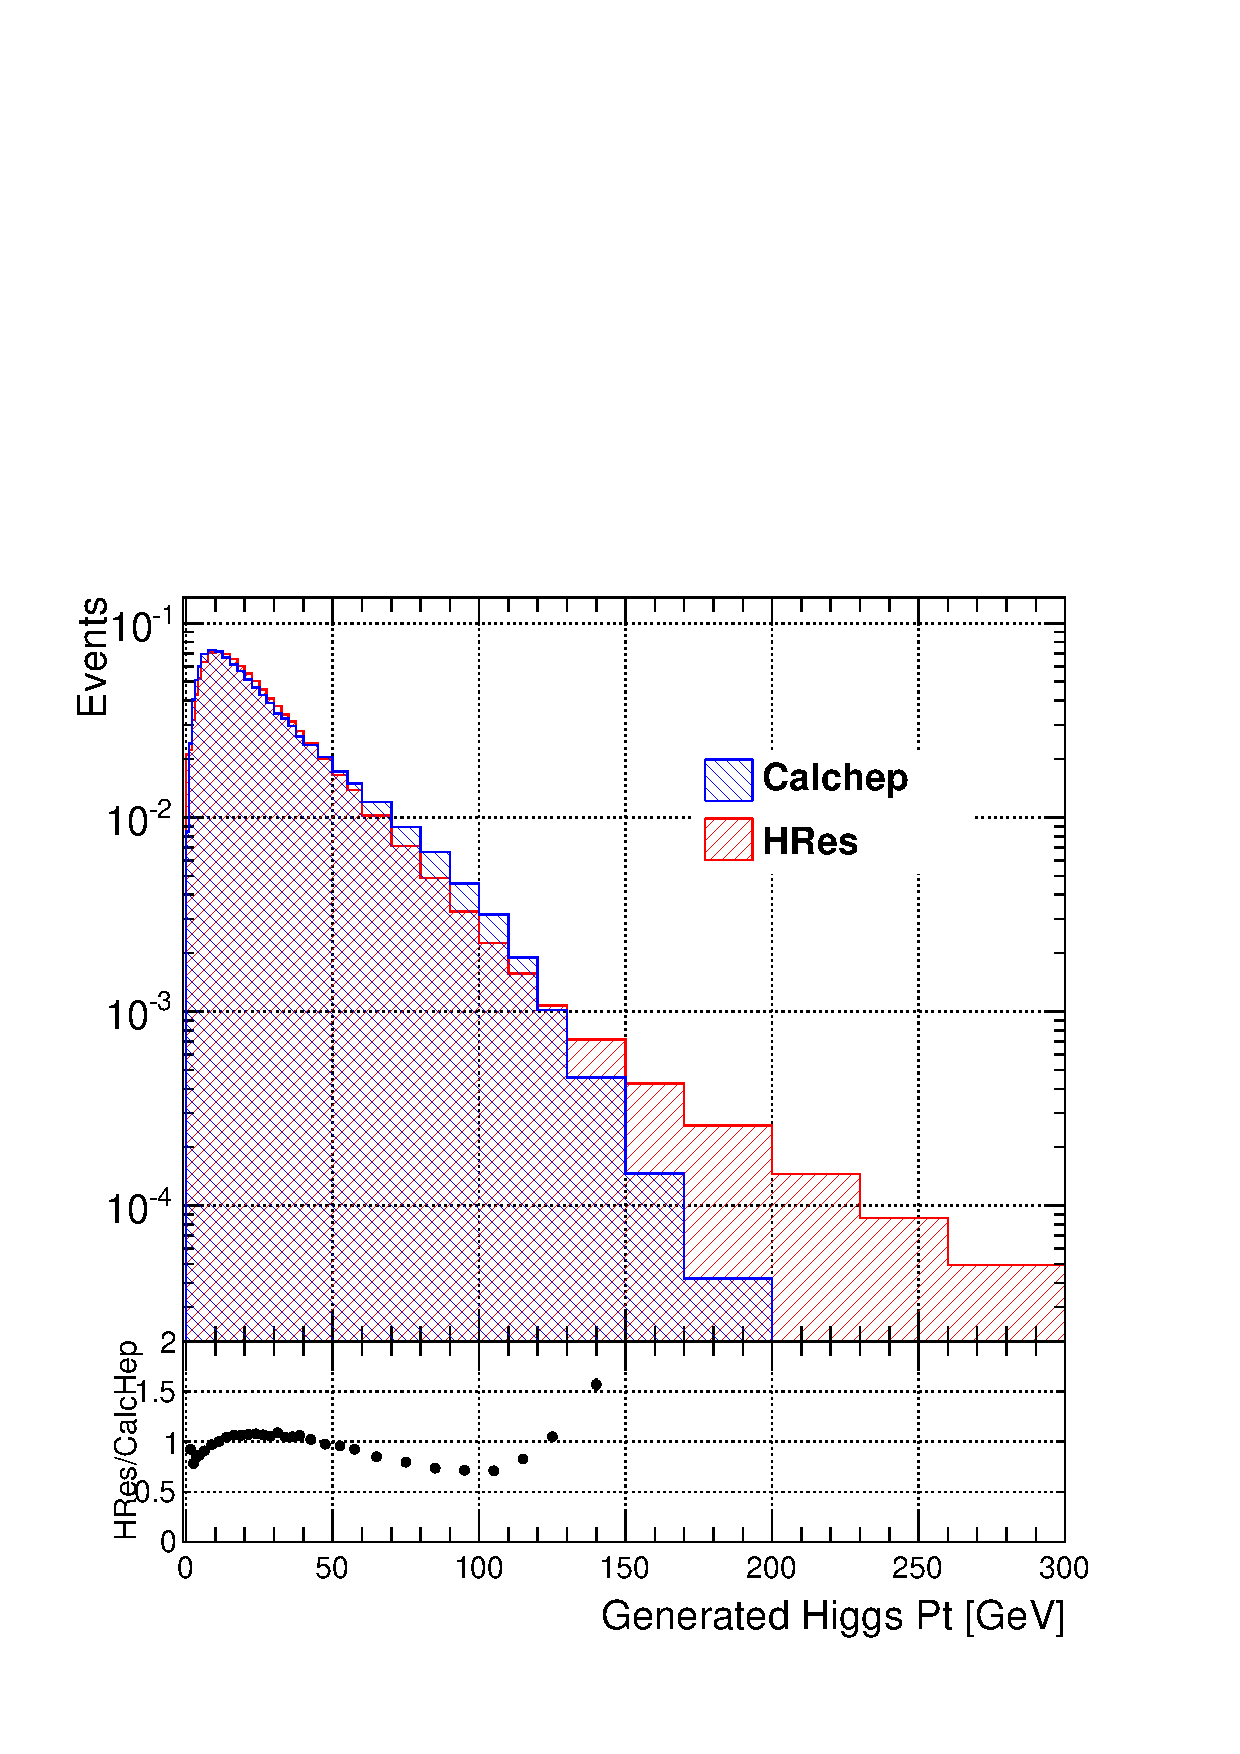
\includegraphics[width=0.45\textwidth]{analysis_figs/shape_gen.pdf}
\caption{The distributions for the generated level Higgs boson \ET and the ratio of the two generators in bins of Higgs Pt to re-weight the events.}
\label{fig:shape_gen}
\end{center}
\end{figure}

Each signal sample is then corrected bin by bin using the ratio. The corrected kinematic distribution along with the kinematic distribution before the correction for the $M_\chi = 120 \GeV$ is shown in Figure~\ref{fig:corrected}. 

\begin{figure}[htb]
\begin{center}
{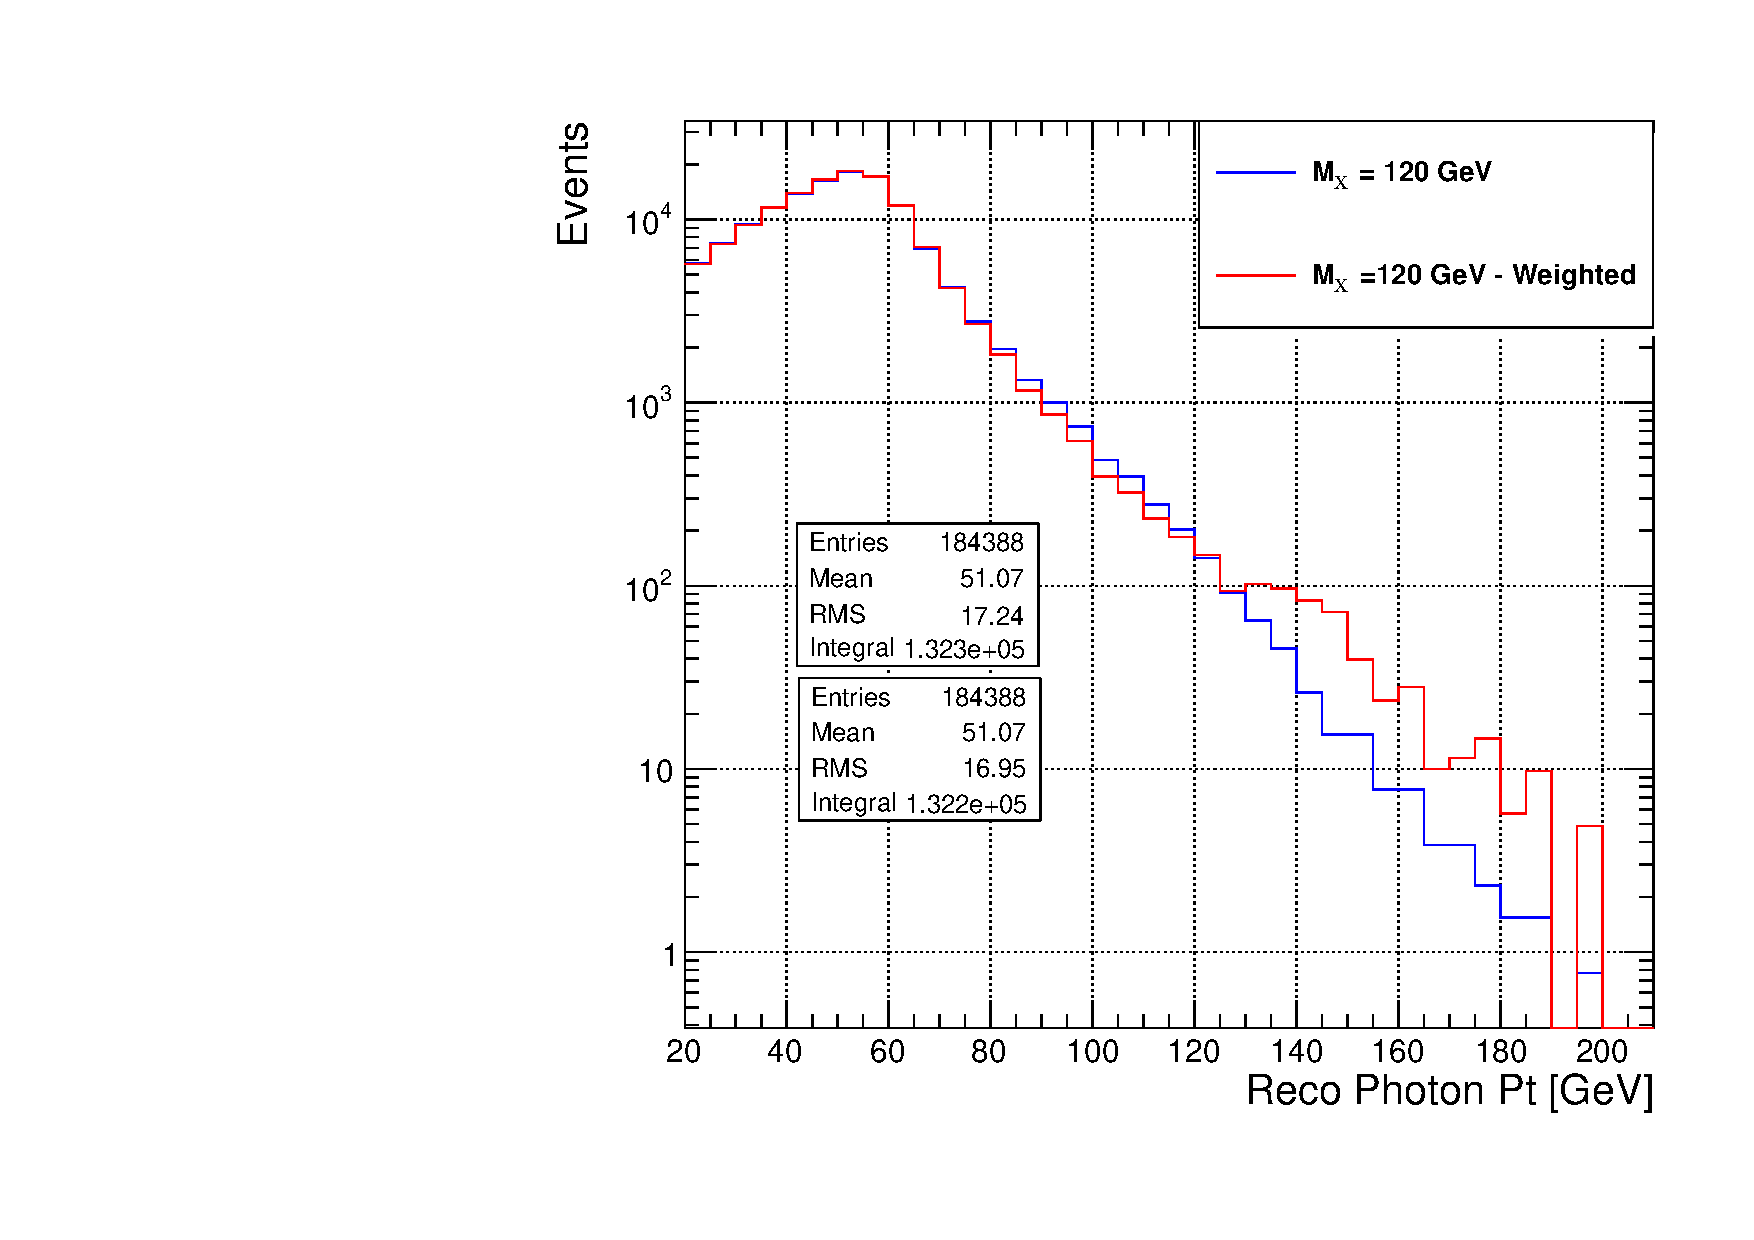
\includegraphics[width=0.45\textwidth]{analysis_figs/signal_photon_reweight.pdf}}\hfill
{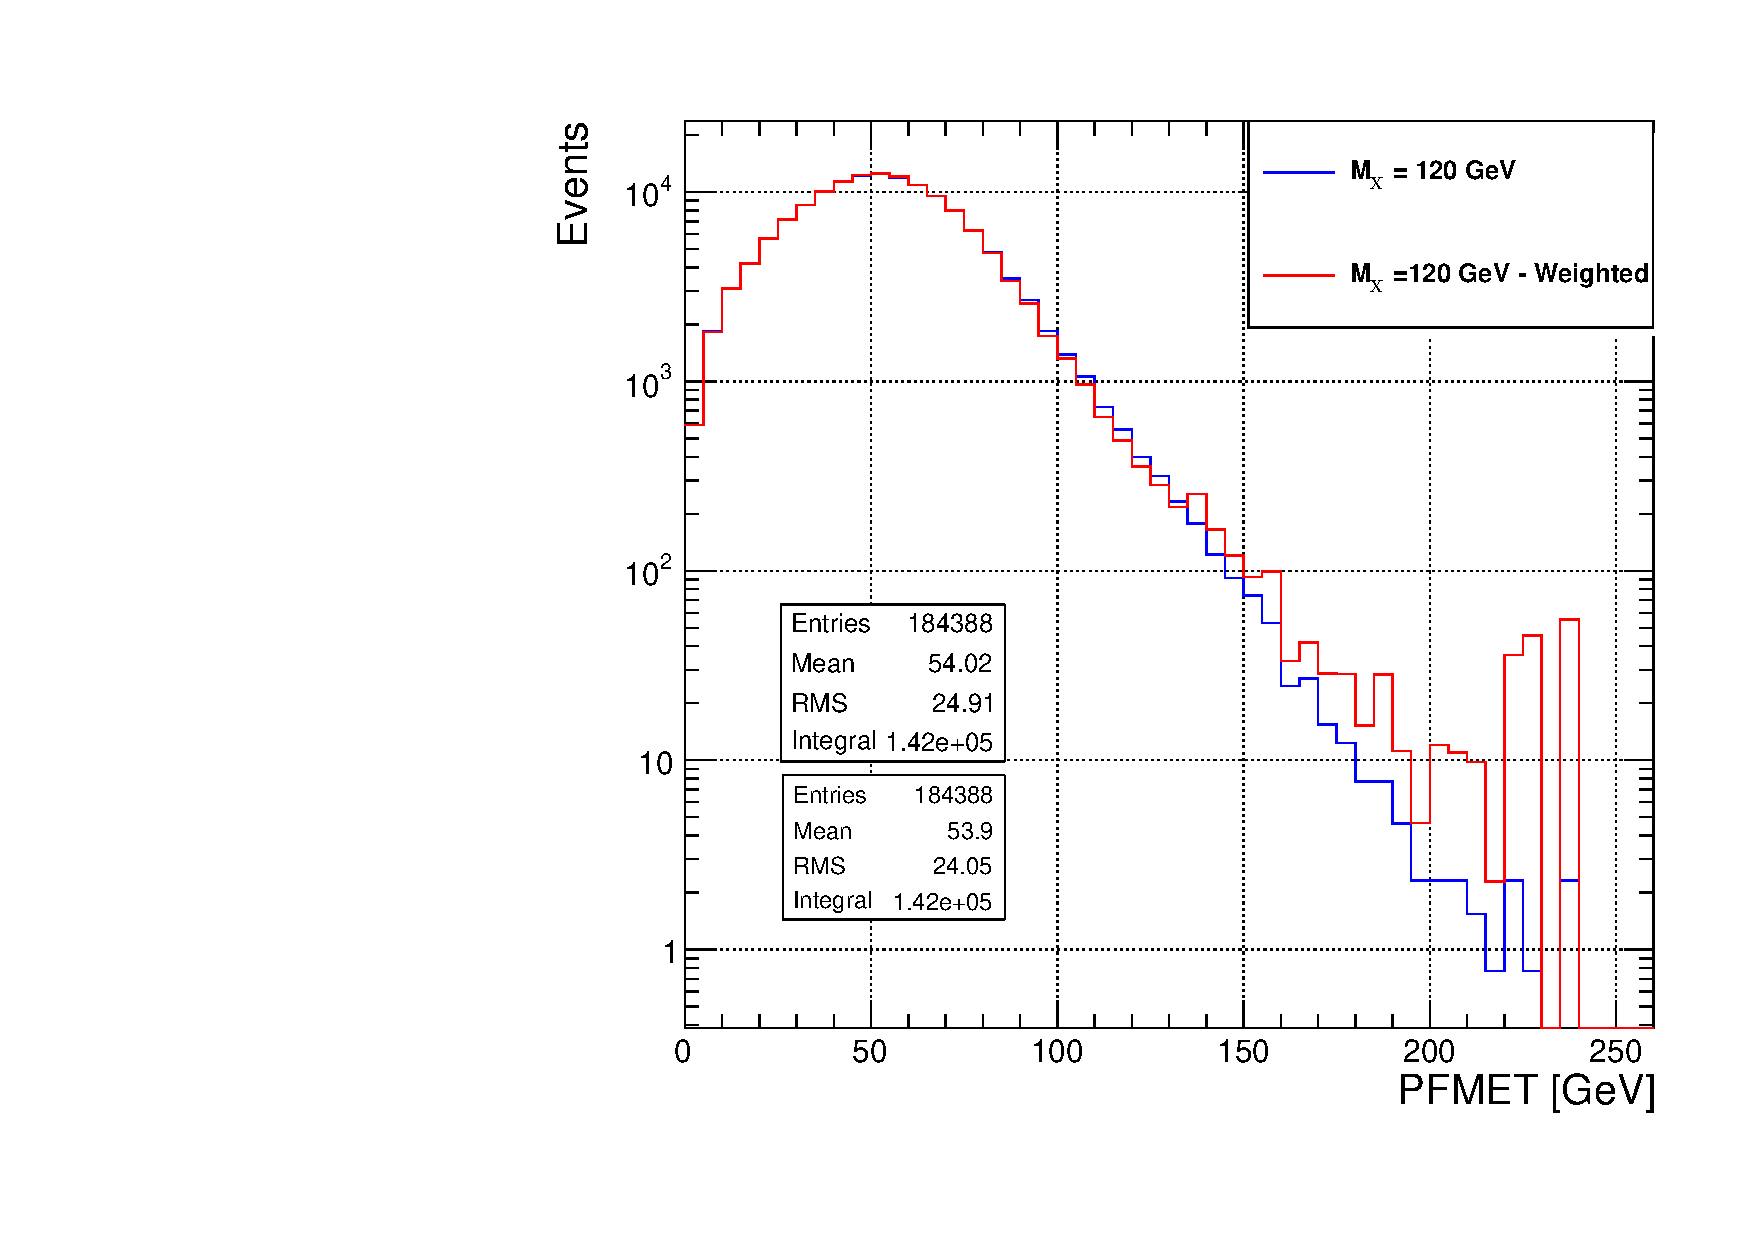
\includegraphics[width=0.45\textwidth]{analysis_figs/signal_met_reweight.pdf}}\hfill
\caption{Photon \ET and \met distribution for the Exotic Higgs Signal Model before and after reweighting}
\label{fig:corrected}
\end{center}
\end{figure}




%The samples for the dark matter signal were made at parton level with \MADGRAPH~\cite{madgraph}. The fragmentation and hadronization was done by \PYTHIA~\cite{pythia}. The parameters used for generating the signal with \MADGRAPH were the mass ($m_{Med}$), width ($\Gamma_{Med}$) and couplings ($g_q$,$g_D$) for the mediator as well as the mass of the dark matter ($m_D$). For the fixed mediator study $m_D = 1$, $10$, $100$, $200$, $300$, $400$, $500$, $700$ GeV while $m_{Med} = 10000$ GeV and $\Gamma_{Med} = 1$ GeV. For the variable mediator study $m_{D}$ = $50$, $500$ GeV, $m_{Med} = 10$, $100$, $300$, $600$, $1000$, $2000$, $3000$, $5000$, $10000$ GeV and $\Gamma_{Med} = m_{Med}/3$, $m_{Med}/10$, $m_{Med}/8\pi$. Both studies use $g_q = 1$ and $g_D = 1$.

\subsection{Pile-Up Reweighting for MC}

The MC samples were generated with pileup interactions to match the expected conditions of each data taking period.
The Deterministic Annealing primary vertex (PV) reconstruction is well-behaved up to high levels of pile up, however the final distribution for the number of reconstructed primary vertices is still sensitive to the details of the primary vertex reconstruction and to differences in the underlying event in data vs MC. The number of reconstructed vertices can further be affected by the event selection criteria and by the trigger.

In order to factorize these effects, instead of reweighting the MC by the number of reconstructed primary vertices, we reweight instead the number of pileup interactions from the simulation truth. The target pileup distribution for data is derived by using the per bunch-crossing-per-luminosity section instantaneous luminosity from the LumiDB together with the total $p-p$ inelastic cross-section to generate an expected pileup distribution, correctly weighted by the  per bunch-crossing-per-luminosity section integrated luminosity over the entire data-taking period \cite{pileup}.

The distribution of the number of vertices in data and MC is shown in Fig.~\ref{fig:vertex} after the above mentioned re-weighting has been applied.

\begin{figure}[htb]
\begin{center}
{\label{fig:NVtx1}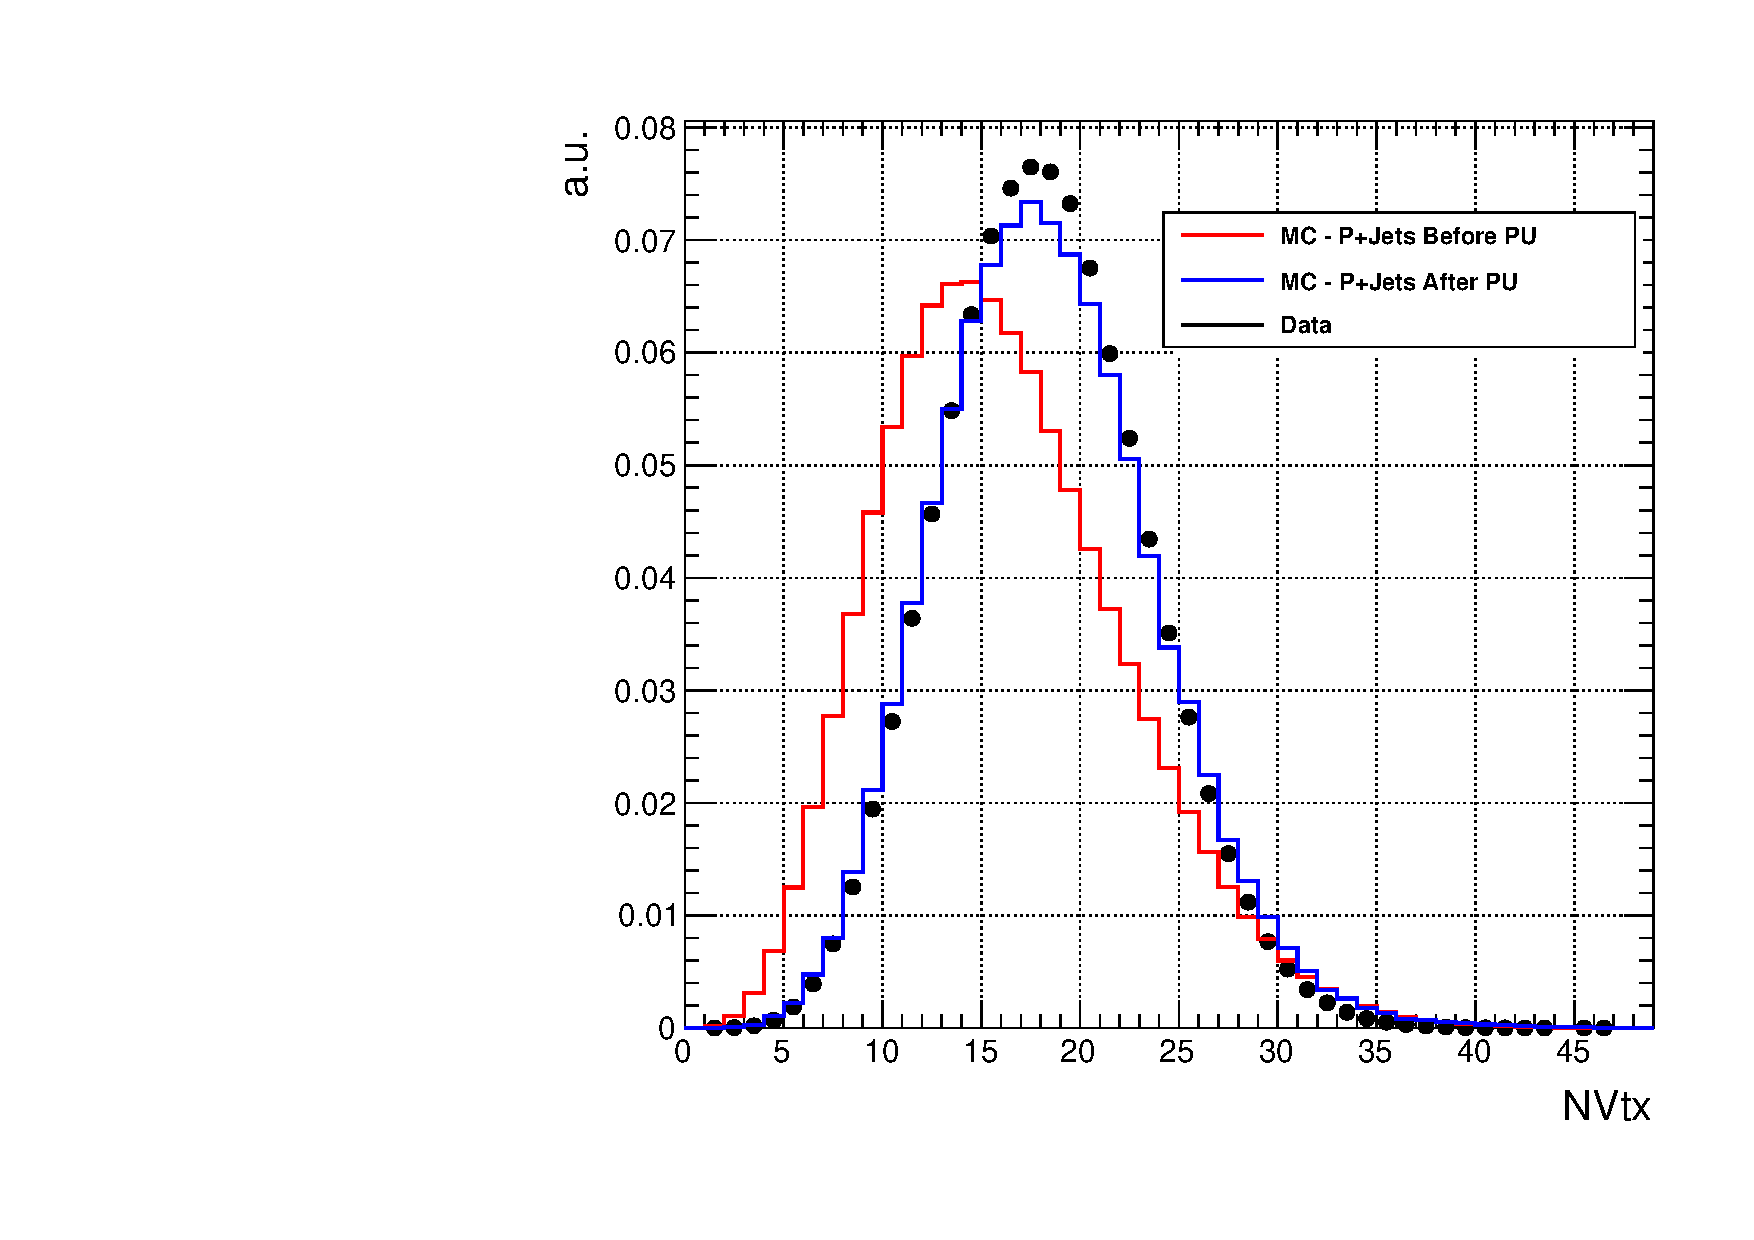
\includegraphics[width=0.45\textwidth]{analysis_figs/nvtx1.pdf}}
{\label{fig:NVtx2}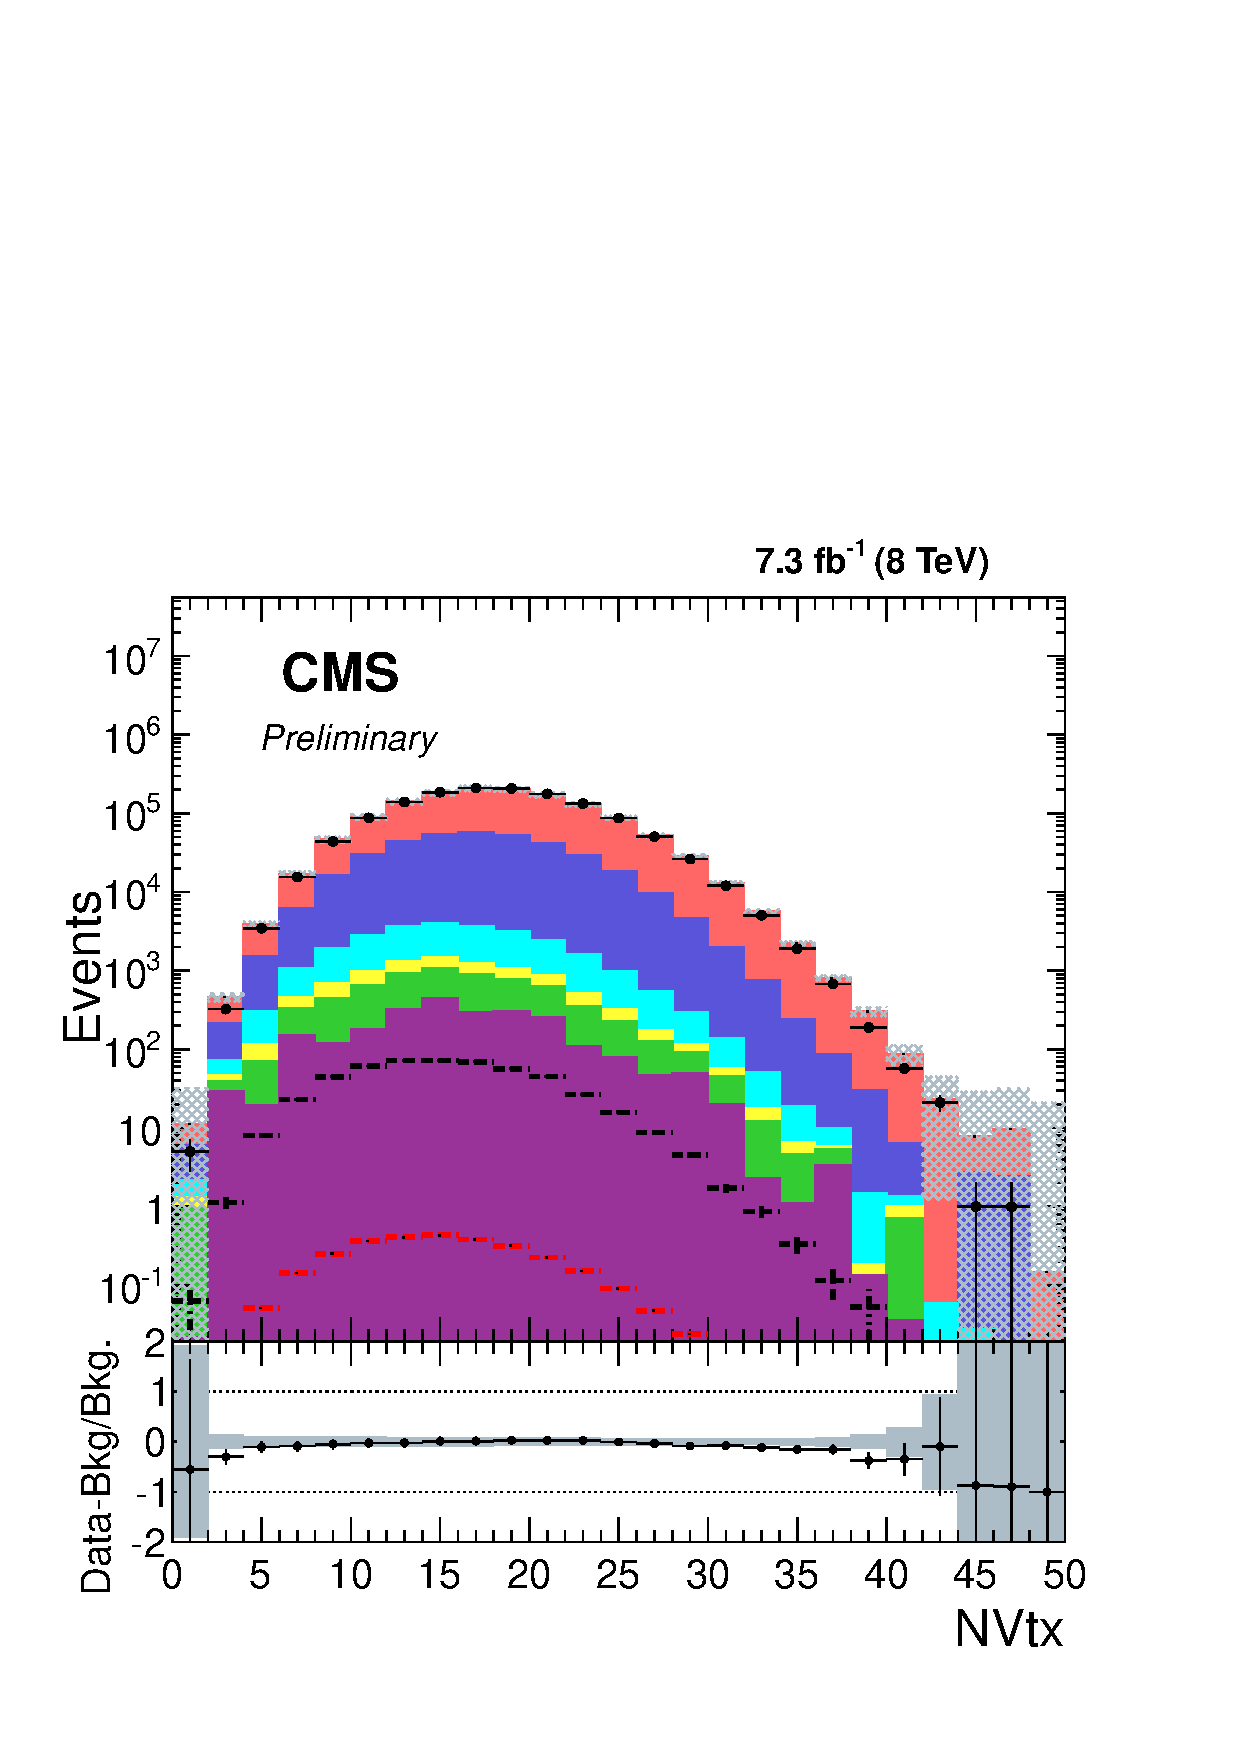
\includegraphics[width=0.45\textwidth]{analysis_figs/nvtx2.pdf}}
\caption{(a) Distribution of the number of vertices in data and Photon + Jets MC before and after the reweighting, both normalized to 1. (b) Distribution of the number of vertices after all our selection for data and background.}
\label{fig:vertex}
\end{center}
\end{figure}

%As it can be seen in our distributions, there seems to be a problem with the reweighting based on the method described above. The excess we see in MC in the high tails is due to the shape seen in the pile up distribution extracted from data as shown in Fig.~\ref{fig:pu_data}~a. Given that the weights for the MC is extracted based on the pile up distribution from data, it is not surprising to be seeing the excess in the tails of MC. The source of this problem is currently unknown and is being investigated. For the time being, we have decided to do a shape normalization for this variable in a region where the signal is $10^5$ times smaller than the total background. We have extracted the reweighting factor by subtracting our data driven backgrounds from the data, and normalizing both the remaining data and total MC distributions to unity and fitting a 6th order polynomial to the ratio of the two distributions. This way we were able to correct the vertex distribution without changing the overall normalization of MC. The corrected distribution is shown in Fig.~\ref{fig:pu_data}~b. 

%\begin{figure}[htb]
%\begin{center}
%{\label{fig:pu_data_a}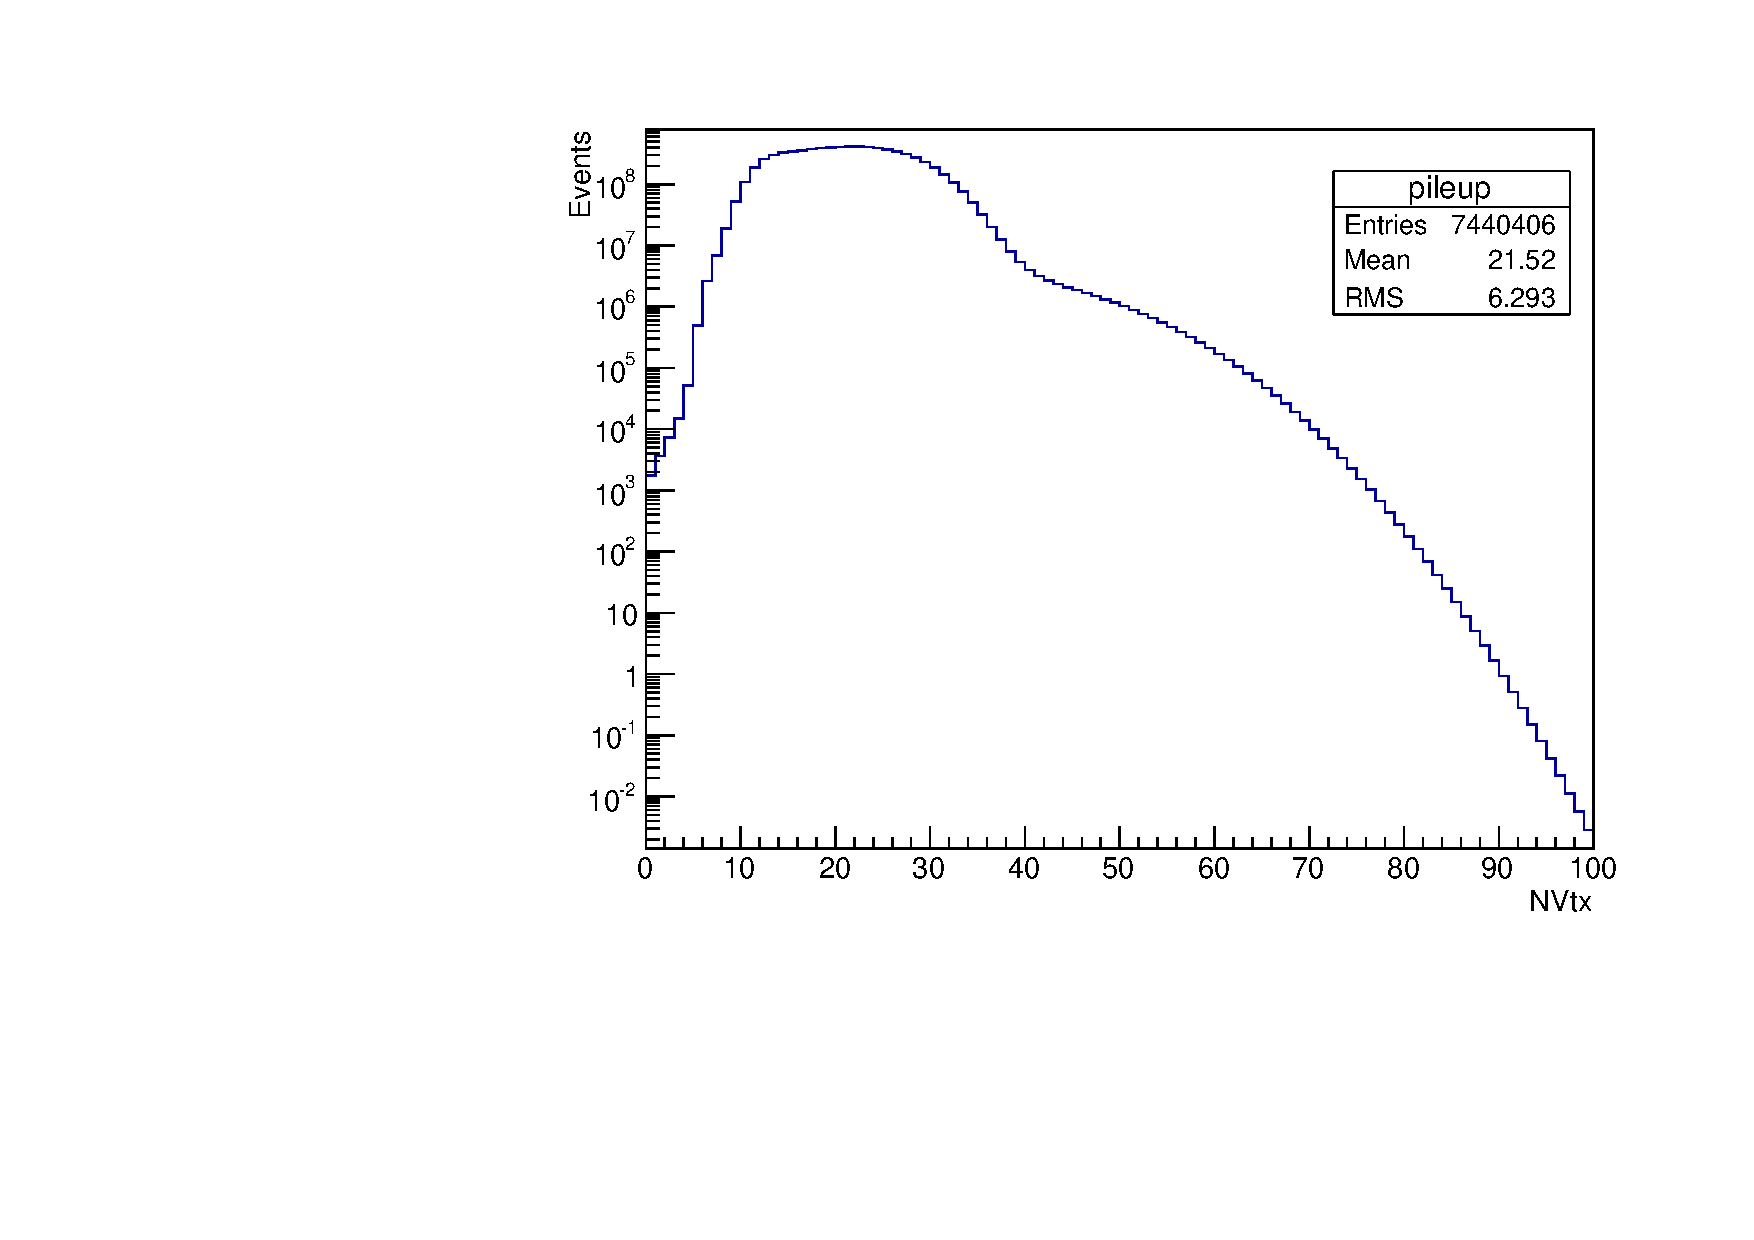
\includegraphics[width=0.45\textwidth]{analysis_figs/pile_up_data.pdf}}
%{\label{fig:pu_data_b}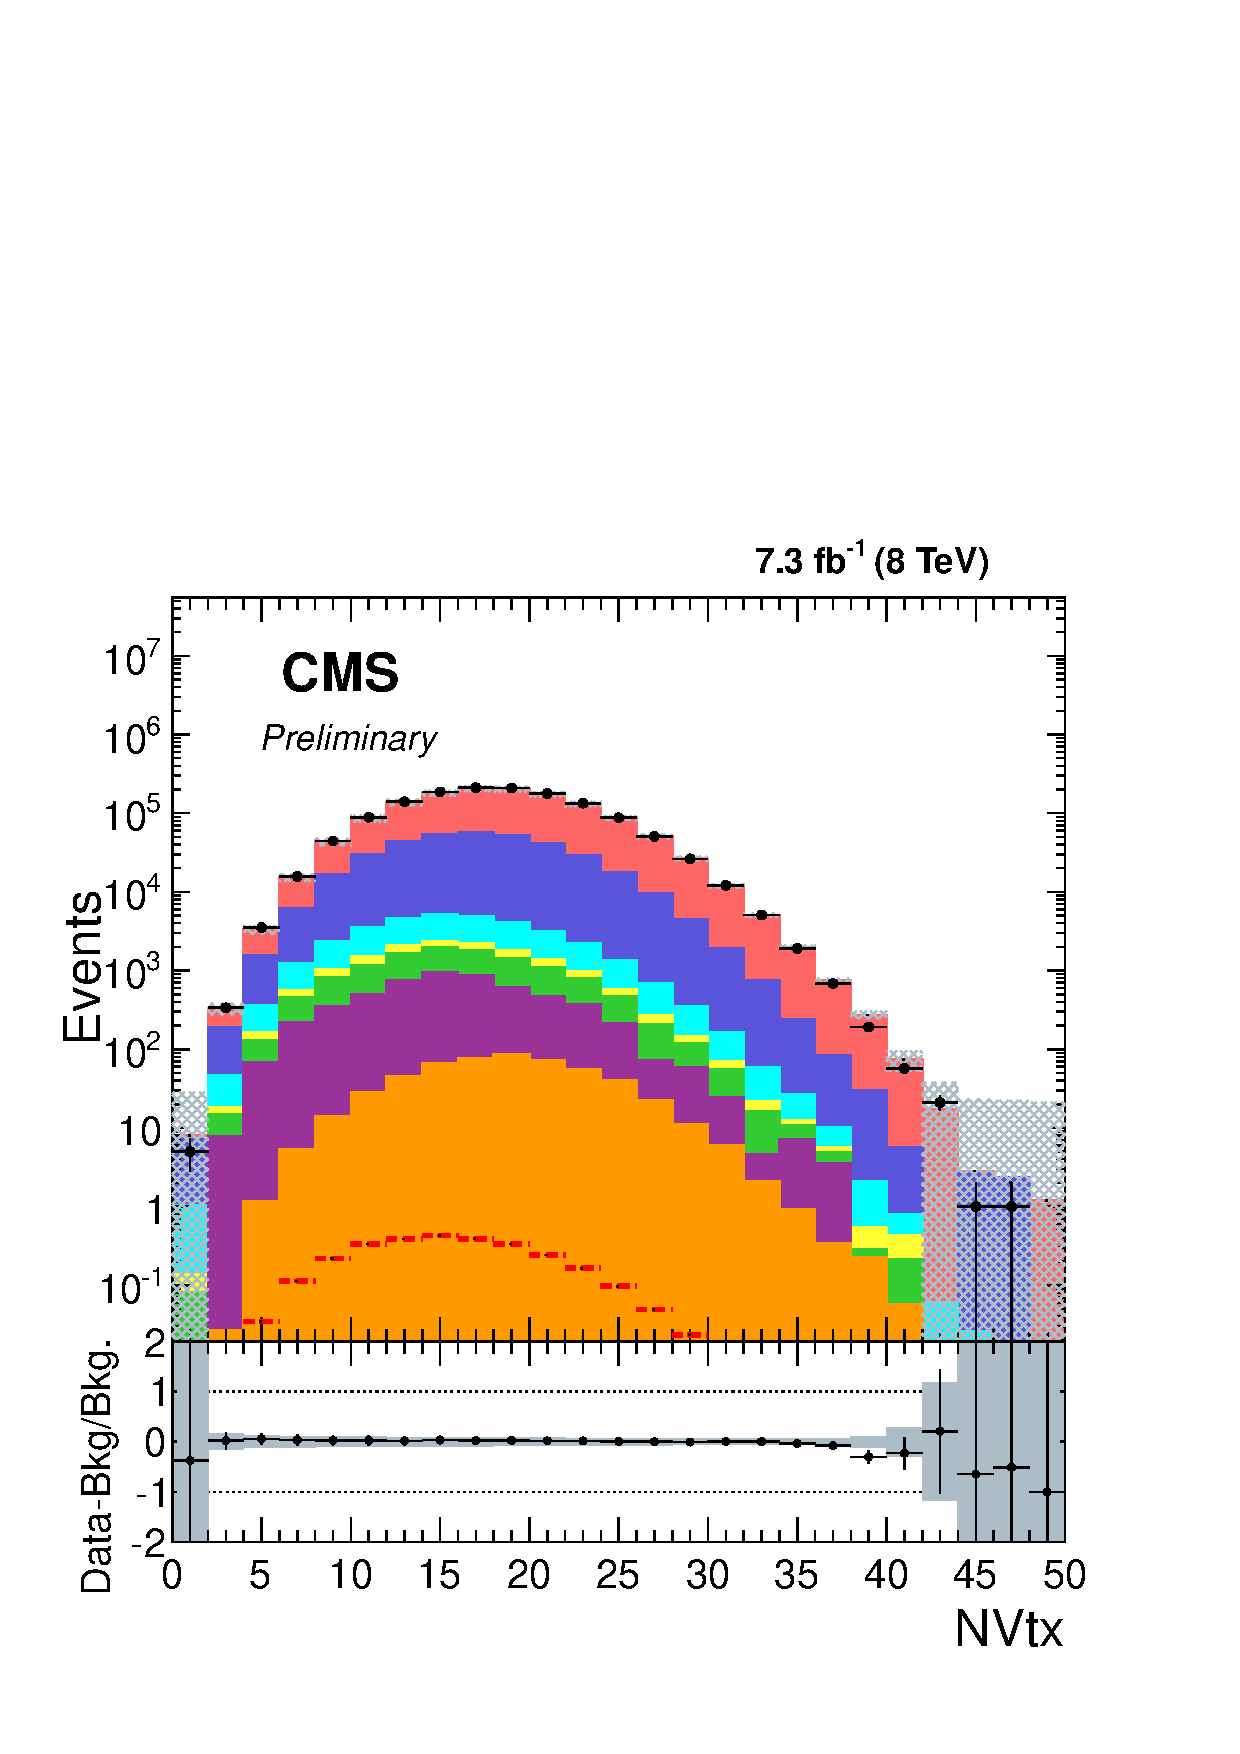
\includegraphics[width=0.45\textwidth]{analysis_figs/nvtx_corr.pdf}}
%\caption{(a) Problematic pile up distribution extracted from data, which is later used to re-weight the MC in the traditional method. (b) Number of vertices distribution after applying a shape re-weighting to the MC based backgrounds.}
%\label{fig:pu_data}
%\end{center}
%\end{figure}


